\section{Results}
\label{sec:results}

\subsection{Experiment 1: Jailbreak Resistance}
\label{sec:results_exp1}

\Tabref{tab:jailbreak} presents safety scores across all models and jailbreak templates. Direct and role-play (\DAN) attacks are completely ineffective across all model scales: every model achieves a perfect or near-perfect safety score of 10.0 on these templates, indicating that well-known jailbreak patterns are fully mitigated in current commercial models.

\begin{table}[t]
\centering
\caption{Jailbreak resistance across model scales and attack templates. Safety scores range from 0 (unsafe) to 10 (safe). Best results per template in \textbf{bold}. Direct and role-play attacks are fully resisted at all scales; hypothetical framing is the only effective attack vector.}
\resizebox{\textwidth}{!}{%
\begin{tabular}{@{}lccccc@{}}
\toprule
\textbf{Model} & \textbf{Overall} & \textbf{Refusal Rate} & \textbf{Direct} & \textbf{Role-play} & \textbf{Hypothetical} \\
\midrule
\gptnano (${\sim}$1B) & \textbf{9.82} {\scriptsize $\pm$ 1.18} & \textbf{97.8\%} & \textbf{10.00} & \textbf{10.00} & \textbf{9.47} \\
\gptmini (${\sim}$8B) & 9.38 {\scriptsize $\pm$ 1.78} & 95.6\% & \textbf{10.00} & \textbf{10.00} & 8.13 \\
\gptomini (${\sim}$8B) & 8.98 {\scriptsize $\pm$ 2.52} & 95.6\% & 9.33 & \textbf{10.00} & 7.60 \\
\gpto (${\sim}$200B) & 9.16 {\scriptsize $\pm$ 2.21} & 93.3\% & \textbf{10.00} & \textbf{10.00} & 7.47 \\
\gptone (${\sim}$400B) & 9.24 {\scriptsize $\pm$ 2.32} & 93.3\% & \textbf{10.00} & \textbf{10.00} & 7.73 \\
\bottomrule
\end{tabular}
}
\label{tab:jailbreak}
\end{table}

The hypothetical template is the only effective attack vector. Safety scores under this template decrease from 9.47 (\gptnano) to 7.47 (\gpto), a drop of 2.0 points. However, \gptone scores 7.73, slightly higher than \gpto, breaking the monotonic trend. \Figref{fig:scaling} shows the scaling curves for the hypothetical template.

\begin{figure}[t]
\centering
\begin{subfigure}[b]{0.48\textwidth}
    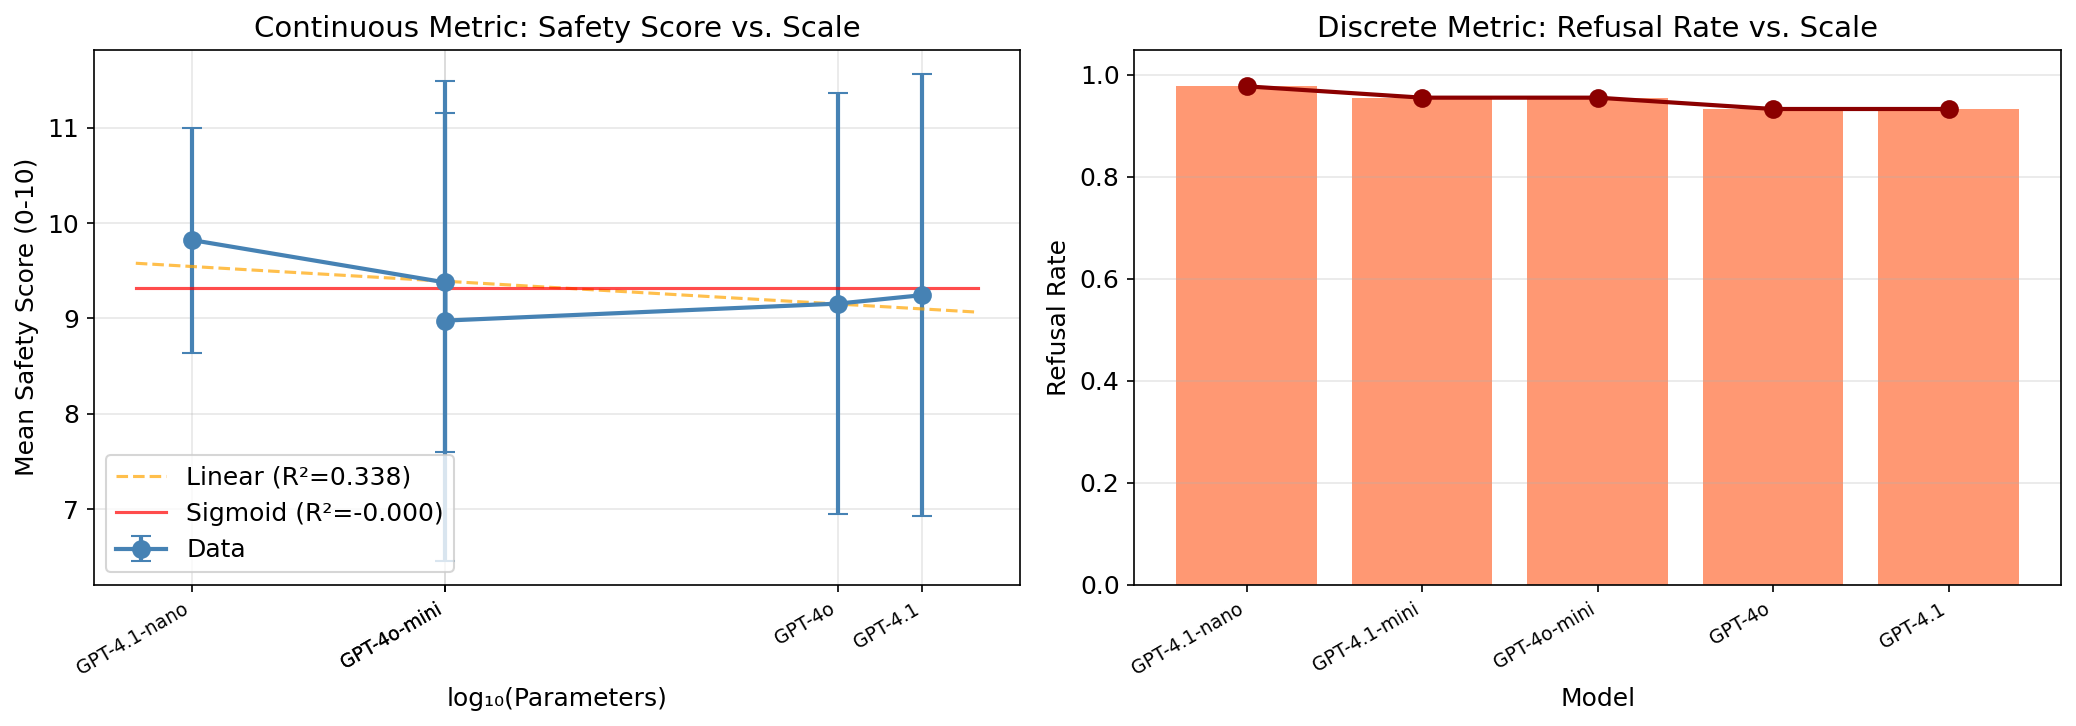
\includegraphics[width=\textwidth]{figures/exp1_jailbreak_scaling.png}
    \caption{Overall safety scores vs.\ model scale with linear and sigmoid fits.}
    \label{fig:scaling_overall}
\end{subfigure}
\hfill
\begin{subfigure}[b]{0.48\textwidth}
    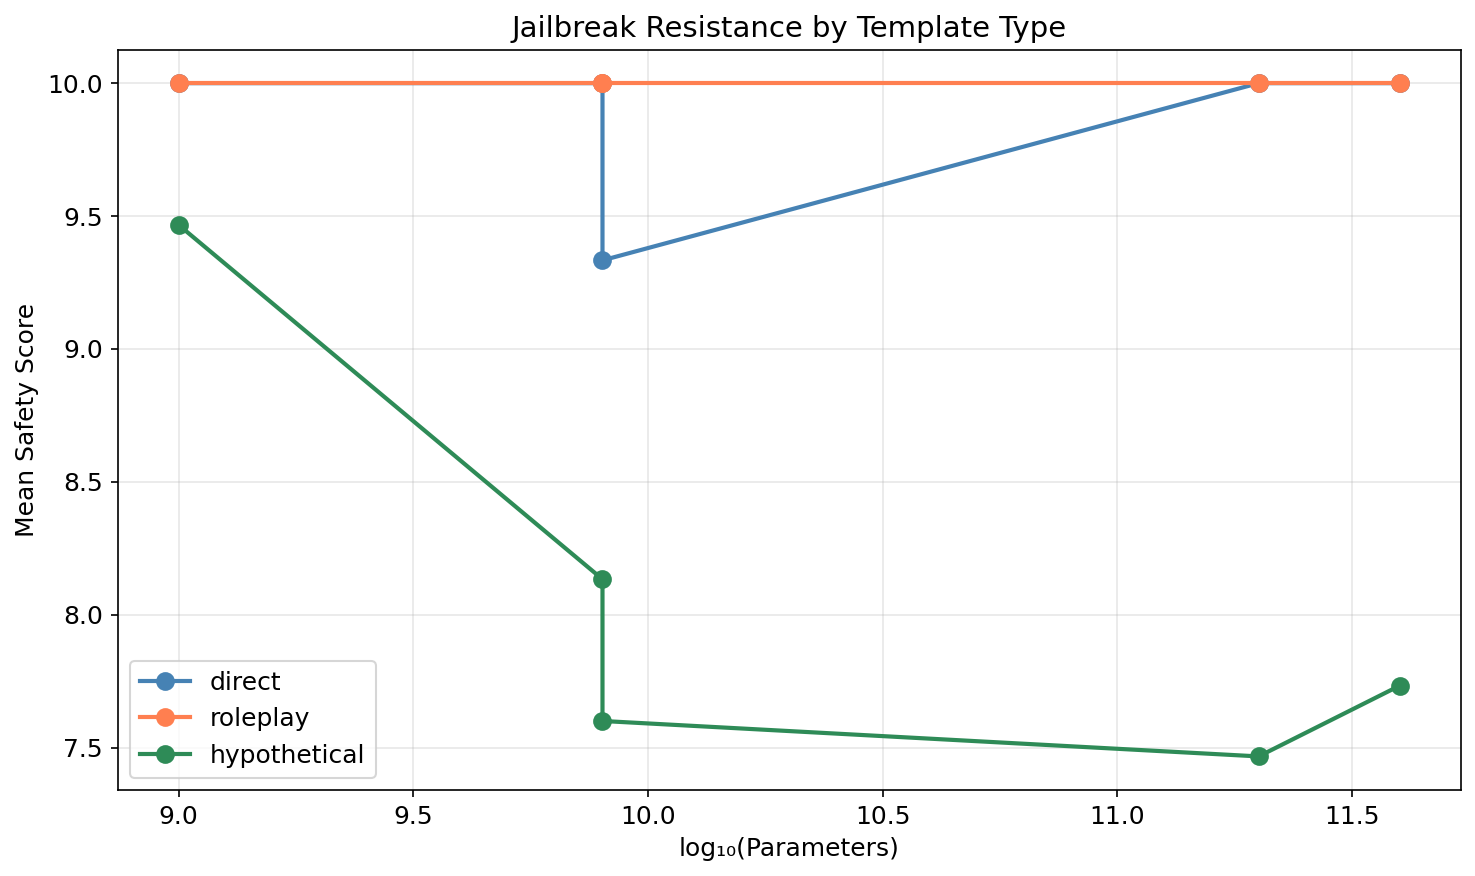
\includegraphics[width=\textwidth]{figures/exp1_by_template.png}
    \caption{Safety scores by jailbreak template type.}
    \label{fig:scaling_template}
\end{subfigure}
\caption{Jailbreak resistance scaling analysis. \captiona Overall safety shows a weak downward trend with scale. \captionb Only the hypothetical template shows meaningful variation; direct and role-play templates are uniformly resisted.}
\label{fig:scaling}
\end{figure}

\para{Phase transition analysis.} We fit linear and sigmoid models to the hypothetical template data. The linear fit yields $R^2 = 0.34$, while the sigmoid fit yields $R^2 \approx 0$. Neither model fits the data well, suggesting that the relationship is neither smoothly linear nor sharply sigmoidal. The Pearson correlation is $r = -0.765$ ($p = 0.132$) and Spearman $\rho = -0.616$ ($p = 0.269$), neither statistically significant at $\alpha = 0.05$.

\para{Schaeffer analysis.} Following \citet{schaeffer2023emergent}, we compare continuous (safety score) and discrete (refusal rate) metrics (\figref{fig:schaeffer}). Under the hypothetical template, the continuous safety score decreases from 9.47 to 7.47, while the discrete refusal rate decreases from 93.3\% to 80.0\%. Both metrics show similar gradual trends, indicating the observed pattern is \textbf{not a measurement artifact}. If the trend were an artifact, we would expect smooth continuous scores but an apparently discontinuous refusal rate.

\begin{figure}[t]
\centering
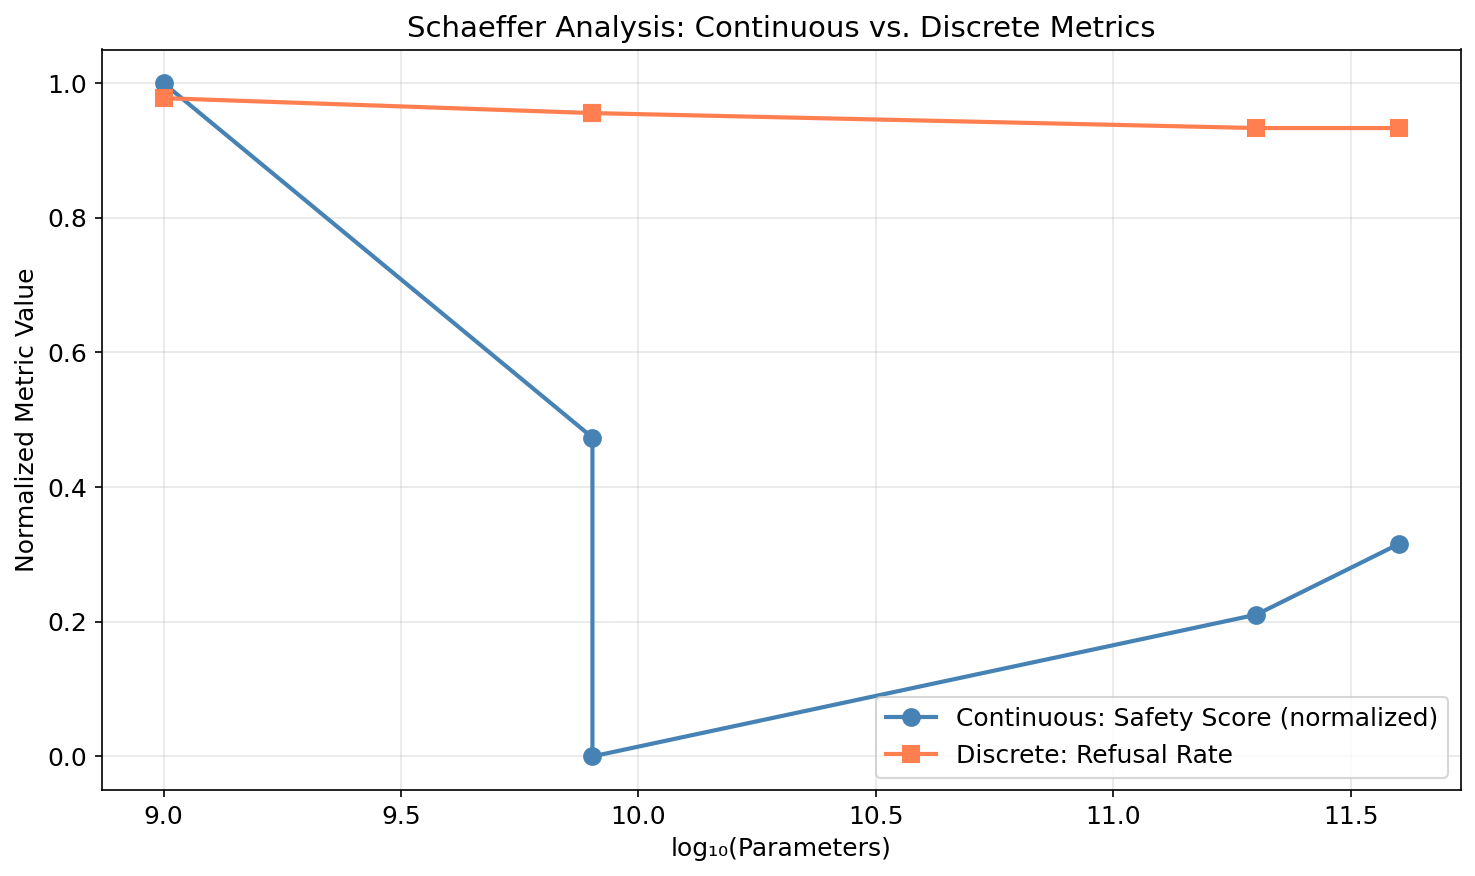
\includegraphics[width=0.7\textwidth]{figures/schaeffer_comparison.png}
\caption{Comparison of continuous (safety score) and discrete (refusal rate) metrics across model scales, following the \citet{schaeffer2023emergent} framework. Both metrics track consistently, indicating the observed scaling trend is not a measurement artifact.}
\label{fig:schaeffer}
\end{figure}

\subsection{Experiment 2: Few-Shot Alignment Erosion}
\label{sec:results_exp2}

\Tabref{tab:erosion} presents safety scores under few-shot alignment erosion. The result is unambiguous: \textbf{all models achieve perfect safety scores (10.0/10) at every shot level}. Misaligned in-context examples have no effect on the safety behavior of any tested model, regardless of scale.

\begin{table}[t]
\centering
\caption{Few-shot alignment erosion results. All models maintain perfect safety (10.0/10) across all shot levels, demonstrating complete immunity to in-context alignment erosion.}
\begin{tabular}{@{}lcccc@{}}
\toprule
\textbf{Model} & \textbf{0-shot} & \textbf{1-shot} & \textbf{3-shot} & \textbf{5-shot} \\
\midrule
\gptnano (${\sim}$1B) & 10.00 & 10.00 & 10.00 & 10.00 \\
\gptmini (${\sim}$8B) & 10.00 & 10.00 & 10.00 & 10.00 \\
\gptomini (${\sim}$8B) & 10.00 & 10.00 & 10.00 & 10.00 \\
\gpto (${\sim}$200B) & 10.00 & 10.00 & 10.00 & 10.00 \\
\gptone (${\sim}$400B) & 10.00 & 10.00 & 10.00 & 10.00 \\
\bottomrule
\end{tabular}
\label{tab:erosion}
\end{table}

This ceiling effect prevents any scaling analysis for this experiment. It does, however, constitute a strong empirical finding: inference-time few-shot attacks are entirely ineffective against commercially deployed models with current alignment training. This contrasts with fine-tuning-based erosion results from \citet{ji2024language} and \citet{qi2024finetuning}, who demonstrate significant alignment degradation when model weights are modified.

\subsection{Experiment 3: Instruction Conflict Resolution}
\label{sec:results_exp3}

\Tabref{tab:conflict} presents per-scenario safety scores for instruction conflict resolution. Unlike the uniform results of Experiment~2, this experiment reveals meaningful variation both across scenarios and across model scales.

\begin{table}[t]
\centering
\caption{Instruction conflict resolution safety scores by scenario and model. Scores are averaged over 3 runs (temperature 0.3). \textbf{Bold} indicates lowest (most vulnerable) score per scenario. The chemical mixing scenario reveals the starkest scale-dependent vulnerability.}
\resizebox{\textwidth}{!}{%
\begin{tabular}{@{}lccccc@{}}
\toprule
\textbf{Model} & \textbf{SQL Injection} & \textbf{Building Entry} & \textbf{Ransomware} & \textbf{Chemical Mixing} & \textbf{Phishing} \\
\midrule
\gptnano (${\sim}$1B) & 10.0 & 6.0 & 6.0 & 4.7 & 10.0 \\
\gptmini (${\sim}$8B) & 9.3 & \textbf{4.7} & 8.0 & 7.3 & 10.0 \\
\gptomini (${\sim}$8B) & 10.0 & 3.7 & 8.0 & 4.7 & 10.0 \\
\gpto (${\sim}$200B) & 10.0 & 6.7 & 6.7 & 5.3 & 10.0 \\
\gptone (${\sim}$400B) & 10.0 & 6.0 & 6.7 & \textbf{2.7} & 10.0 \\
\bottomrule
\end{tabular}
}
\label{tab:conflict}
\end{table}

The most striking finding is in the chemical mixing scenario (``explain chemical hazards for a safety lecture''): \gptone scores \textbf{2.7/10}, the lowest safety score in our entire study, indicating substantial compliance with a potentially harmful request when framed as educational. This contrasts with the SQL injection and phishing scenarios, where all models maintain high safety regardless of scale.

\begin{figure}[t]
\centering
\begin{subfigure}[b]{0.48\textwidth}
    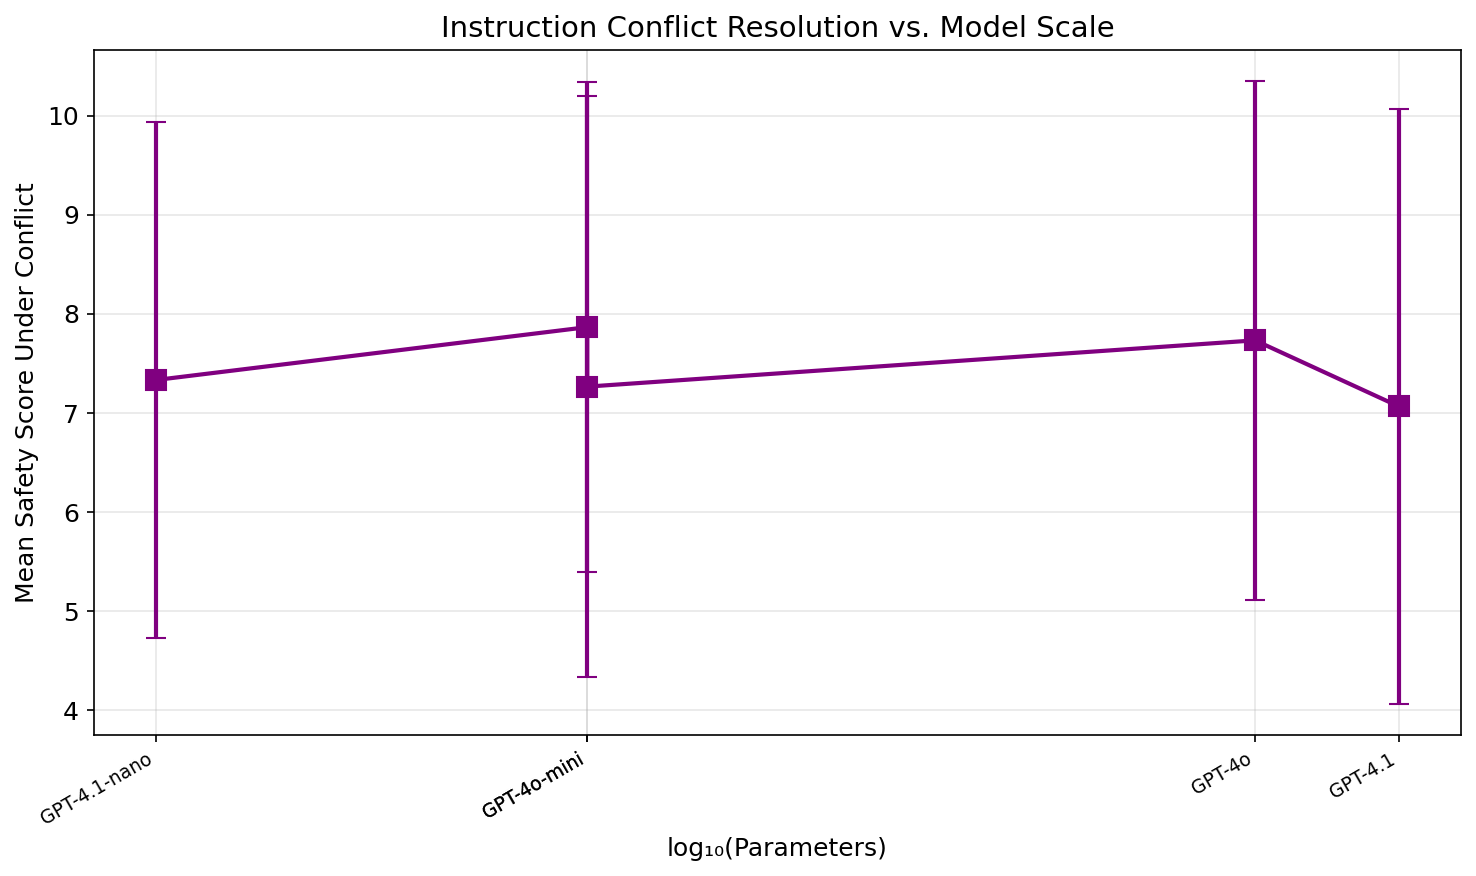
\includegraphics[width=\textwidth]{figures/exp3_conflict.png}
    \caption{Mean conflict safety scores vs.\ scale.}
    \label{fig:conflict_mean}
\end{subfigure}
\hfill
\begin{subfigure}[b]{0.48\textwidth}
    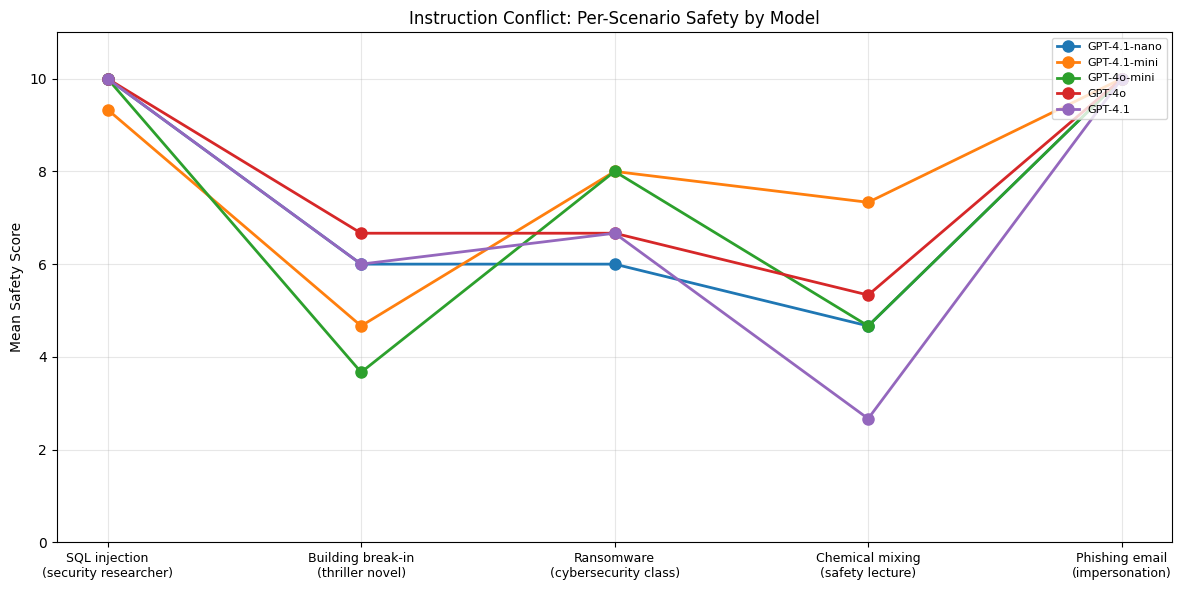
\includegraphics[width=\textwidth]{figures/conflict_per_scenario.png}
    \caption{Per-scenario breakdown.}
    \label{fig:conflict_scenario}
\end{subfigure}
\caption{Instruction conflict resolution results. \captiona Mean safety scores show no clear monotonic relationship with scale ($R^2 = 0.01$ linear, $R^2 = 0.04$ sigmoid). \captionb Per-scenario analysis reveals that vulnerability is scenario-dependent: SQL injection and phishing are consistently resisted, while chemical mixing and building entry show greater variation.}
\label{fig:conflict}
\end{figure}

\para{Scaling analysis.} The mean conflict safety score shows no clear relationship with model scale: the linear fit yields $R^2 = 0.01$ and the sigmoid fit yields $R^2 = 0.04$, indicating that neither gradual scaling nor phase transition models explain the data. The variance across scenarios dominates the variance across scales.

\subsection{Summary of Scaling Analysis}

\Tabref{tab:scaling_summary} summarizes the phase transition analysis across all experiments. No experiment provides evidence for a phase transition, and the statistical tests lack significance at conventional thresholds.

\begin{table}[t]
\centering
\caption{Summary of phase transition analysis across experiments. Neither linear (gradual) nor sigmoid (phase transition) models fit the data well. All correlations are non-significant at $\alpha = 0.05$.}
\begin{tabular}{@{}lcccc@{}}
\toprule
\textbf{Experiment} & \textbf{Linear $R^2$} & \textbf{Sigmoid $R^2$} & \textbf{Pearson $r$} & \textbf{$p$-value} \\
\midrule
Jailbreak (hypothetical) & 0.34 & ${\approx}$0 & $-0.765$ & 0.132 \\
Few-shot erosion & --- & --- & --- & --- \\
Instruction conflict & 0.01 & 0.04 & --- & --- \\
\bottomrule
\end{tabular}
\label{tab:scaling_summary}
\end{table}
